\documentclass[crop,tikz,convert={outext=.svg,command=\unexpanded{pdf2svg \infile\space\outfile}}]{standalone}

\usepackage{pgfplots}
\tikzset{>=latex}
\usetikzlibrary{decorations.markings}
\pgfplotsset{compat=1.16}

\begin{document}
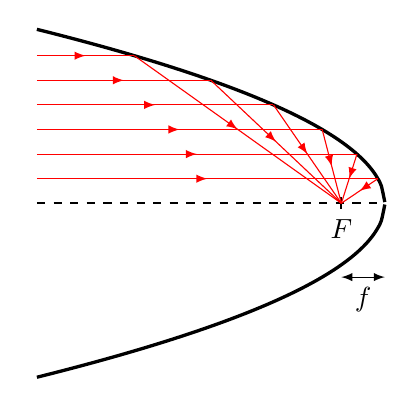
\begin{tikzpicture}
  \begin{axis}[
    width=6cm,
    height=6cm,
    domain=-2:0,
    samples=100,
    axis y line=middle,
    axis x line=middle,
    axis line style={draw=none},
    tick style={draw=none},
    xticklabels=\empty,
    yticklabels=\empty,
    clip=false
    ]
    \addplot[smooth,very thick] {  sqrt(-x) };
    \addplot[smooth,very thick] { -sqrt(-x) };
    \draw[thick,dashed] (axis cs:-2,0) -- (axis cs:0,0);
    \draw[thick] (axis cs:-0.25,0.05) -- (axis cs:-0.25,-0.05) node[below] {$F$};
    \draw[<->] (axis cs:-0.25,-0.6) -- node[below] {$f$} (axis cs:0,-0.6);
    \begin{scope}[decoration={
        markings,
        mark=at position 0.5 with {\arrow{>}}}
      ]
      \pgfplotsinvokeforeach{1.2,1,...,0.2}{%
        \draw[red,postaction={decorate}] (axis cs:-2,#1) -- (axis cs:{-#1*#1},#1);
        \draw[red,postaction={decorate}] (axis cs:{-#1*#1},#1) -- (axis cs:-0.25,0);
      }
    \end{scope}
  \end{axis}
\end{tikzpicture}
\end{document}
